\documentclass[main.tex]{subfiles}
\begin{document}
    \chapter{Next Steps}
    \label{ch:next-steps}
    We have split this competition year broadly into three "phases," corresponding to the University of Waterloo's academic terms.
    
    \section{Design Phase, Aug 2017 - Jan 12, 2017}
    We outline the accomplishments during this phase in \hyperref[ch:intro]{the Introduction}.
    
    \section{Build Phase, Jan 2017 - Apr 2017}
    The second phase, the Build Phase, starts directly after the FDP submission; the plan is to have functioning and well-tested separate subsystems by April. Additionally, we have set a goal of \$100,000 in sponsorship from companies in Canada and outside, leaving room for unplanned technical expenses. We think this goal will be relatively easy to reach, allowing us to put additional resources toward side projects such as building a several-hundred-foot test track, investigating a Linear Induction Motor design for Competition 4, and building a stronger outreach program. (\hyperref[app:bom]{Appendix \ref{app:bom}} on page \pageref{app:bom} provides cost estimates of all the components of the pod.)
    
	\section{Test Phase, May 2017 - ???}
    The third phase, the Test Phase, will primarily be the full assembly of the pod and performing all full-pod tests. As we don't know the exact date of the next Hyperloop Competition, we're not able to plan this in too much detail. However, if the competition is again in August, we're planning on completing all the checklists and inspections outlined in the Safety and Testing Checklist ourselves before we step foot in California.
    
    \section{Pod Production Schedule}
    We plan on spending the next few weeks sourcing parts and performing any additional design improvements as suggested by SpaceX.
    
    \section{Testing}
    Component and system test program before the Pod arrives for the Competition - summary of all tests [COMPILE THIS FROM OTHER PARTS]
    
    The overall purpose of testing is to verify that the friction drive will be able to function as per design intent. This involves examining certain critical components that may have failure modes that will be detrimental to the functionality of the pod, on or off the track. Testing will also be done to validate certain principles that will be vital to ensuring that the function as per design intent. Some values or concepts are hard to obtain numerically or theoretically, and require empirical testing in order to obtain such. Testing will also reveal flaws in design, and will allow us to fix these flaws, in order to be prepared and safe before we enter the competition.\\
    
    Three different testings are done:
    \begin{itemize}
        \item Motor dynamometer
        \item Wheel endurance testing
        \item Vibration testing
    \end{itemize}

   \begin{figure}
		\centering
       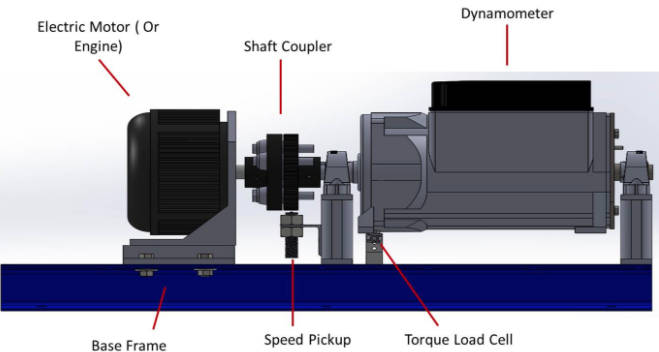
\includegraphics[width=0.5\linewidth]{images/motordyna}
       \caption{Motor Dynamometer}
       \label{fig:motordyna}
   \end{figure}
    A test needs to be conducted with a motor dynamometer (\reffig{fig:motordyna}) to obtain empirical values on motor performance in terms of:
    
    \begin{itemize}
        \item torque/power
        \item RPM ranges
        \item heat generation and thermal profile
        \item power draw (voltage and current)
        \item ESC functionality
        \item power delivery efficiency
    \end{itemize}
    
    Motor performance will be improved by analyzing power/torque curves and optimizing ESC control in order to create a custom map that fits our gear reduction system and acceleration profile. In addition, it allows us to discover and troubleshoot failure modes creates due to design specifications.\\
    
    Moreover, a test to ensure a sufficient endurance level for the wheels is completed. It is crucial to verify that the wheels are able to handle our loads and RPM ranges. A tread wear analysis would be done during acceleration profile and braking phase. A vibration analysis will also be completed to testify that the wheels are two plane balanced.\\

    Furthermore, a vibration test (\reffig{fig:vibra}) will be conducted to test the damping and spring performance and characteristics of the system. This allows us to obtain empirical values of the pod acceleration and position. The analysis provides us with the needed information to tune the suspension to achieve critical damping, and to discover and troubleshoot suspension failure modes.\\

     \begin{figure}
           \centering
       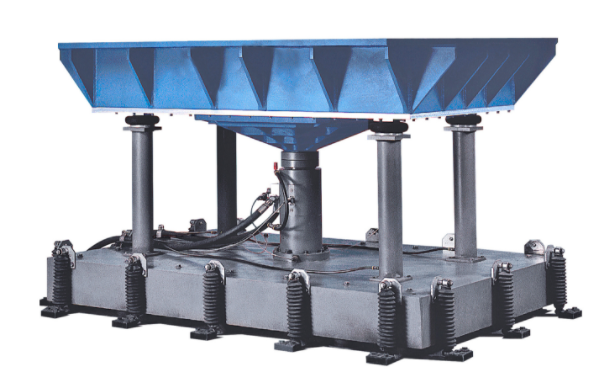
\includegraphics[width=0.5\linewidth]{images/vibra}
       \caption{Vibration testing}
       \label{fig:vibra}
   \end{figure}
    
    \section{Flywheel Test Rig}
    We do not yet have detailed design for the flywheel test rig, but it is currently underway. We expect the rig to be completed approximately at the same time as subsystems are completed and assembled.
    
	The main test rig involves a flywheel that comes into contact with the drive wheel, which is used to substitute the I-Beam track, in order to test the endurance of the wheel. This rig can also be used to test eddy current braking and lateral systems.\\
    
    Unfortunately, initial investigation revealed that a full speed test (~90m/s) would require an unreasonably large and strong flywheel, which would be extremely expensive and dangerous to design. Therefore, the current design of the test rig is intended to conduct half-speed tests (~45m/s). This provides a cheaper and more realistic design while still obtaining valuable real-world data from which we can test hypotheses and extrapolate useful conclusions.\\
    
    The flywheel is composed of \SI{16}{in} diameter aluminum bar stock, which replicates the material of the I-Beam, along with additional \SI{12}{in} diameter cast iron bar stock that is used to increase the moment of inertia to the required level. The cost of the flywheel and the mount is approximately 1120 CAD in total. The concept design of the test rig is shown in \reffig{fig:testrig}.\\
    
    \begin{figure}
           \centering
   \begin{subfigure}{0.4\textwidth}
       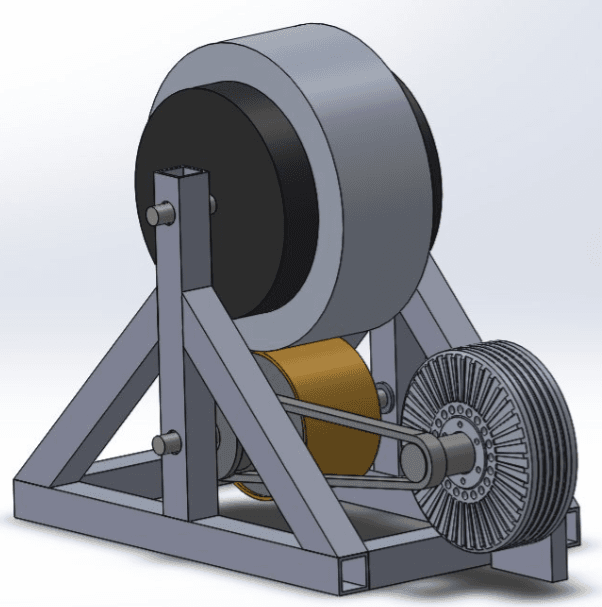
\includegraphics[width=\linewidth]{images/testrig1}
       \caption{}
       \label{fig:testrig1}
       \end{subfigure}        
       \begin{subfigure}{0.4\textwidth}
       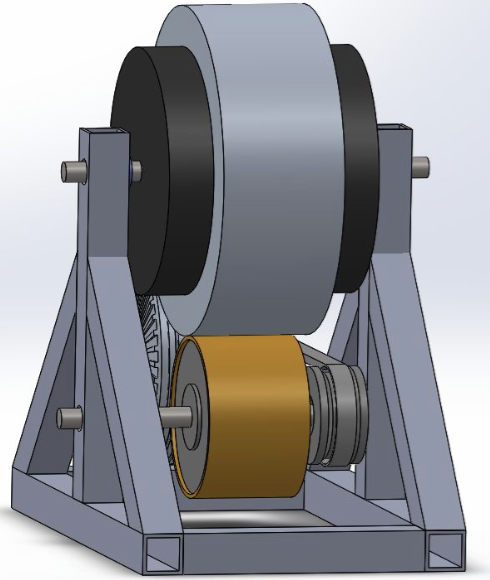
\includegraphics[width=\linewidth]{images/testrig2}
       \caption{}
       \label{fig:testrig2}
       \end{subfigure}
       \caption{CAD views of conceptual test rig design}
       \label{fig:testrig}
   \end{figure}
    
	Since the test rig involves rotating heavy materials at high rotational velocities, safety is critical. A thick protective barrier will be built around the test rig to prevent accidents, such as wheels getting dislodged. In case of emergency, a band brake can be applied to the shaft, which is a simple and reliable solution for braking.\\

\end{document}
